% ============================================================
%  Semana 3 · Clase 5 — Bases de datos relacionales y SQL básico
%  Curso: Análisis y Visualización de Datos para la Toma de Decisiones
%
%  Formato de la sesión (3 h):
%    Hora 1 — Bases de datos relacionales: tabla, registro, campo,
%             clave primaria, esquema relacional (tienda.db)
%    Hora 2 — SQL básico: SELECT, FROM, WHERE, ORDER BY, LIMIT,
%             operadores de comparación y lógicos
%    Hora 3 — Laboratorio: notebooks/lab-sql-basico.ipynb
%             (SQLite sobre "tienda.db", en Google Colab, con guía
%             alterna para DBeaver)
%
%  Compilar (dos veces) directamente desde esta carpeta:
%    xelatex semana03-clase05.tex
%    xelatex semana03-clase05.tex
% ============================================================
\documentclass[aspectratio=169,11pt]{beamer}

\usepackage{../../../plantilla/beamerthemeesumer}
\usetheme{esumer}

\usepackage[spanish]{babel}
\usepackage{booktabs}
\usepackage{graphicx}
\usepackage{listings}

% ---------------- Bloque de código SQL ----------------
\lstdefinelanguage{SQL}{
  morekeywords={SELECT,FROM,WHERE,ORDER,BY,LIMIT,AND,OR,NOT,IN,BETWEEN,LIKE,IS,NULL,ASC,DESC,DISTINCT},
  sensitive=false,
  morecomment=[l]{--},
}
\lstset{
  language=SQL,
  basicstyle=\ttfamily\small,
  keywordstyle=\color{esumerNavy}\bfseries,
  commentstyle=\color{esumerGray!70!black}\itshape,
  stringstyle=\color{esumerTeal},
  backgroundcolor=\color{esumerGray!35},
  frame=single,
  rulecolor=\color{esumerGray},
  framesep=6pt,
  xleftmargin=6pt,
  xrightmargin=6pt,
  breaklines=true,
  showstringspaces=false,
}

% ---------------- DATOS DE LA CLASE ----------------
\title{Bases de datos relacionales y SQL básico}
\subtitle{De preguntarle a un DataFrame a preguntarle a una base de datos}
\author{Docente: Cristian A. Jimenez C., MSc}
\date{Sep 22 al 27}

\setmodulo{Módulo 1: Explorar (Fundamentos y Consulta de Datos)}
\setsemana{3}
\setclase{5}
\setfechaclase{Sep 22 al 27}
\setmodalidad{Virtual}
% -----------------------------------------------------

\graphicspath{{figuras/}}

\begin{document}

{
\setbeamertemplate{footline}{}
\begin{frame}[plain]
  \titlepage
\end{frame}
}

\begin{frame}{Agenda de hoy (3 horas)}
  \begin{columns}[T,onlytextwidth]
    \column{0.32\textwidth}
    \begin{block}{Hora 1}
      \small Bases de datos relacionales: tabla, registro, campo, clave
      primaria y esquema relacional
    \end{block}
    \column{0.32\textwidth}
    \begin{block}{Hora 2}
      \small SQL básico: \texttt{SELECT}, \texttt{FROM}, \texttt{WHERE},
      \texttt{ORDER BY}, \texttt{LIMIT} y operadores
    \end{block}
    \column{0.32\textwidth}
    \begin{block}{Hora 3}
      \small Laboratorio: consultas de extracción y filtrado sobre una
      base de datos empresarial
    \end{block}
  \end{columns}
  \vspace{0.4cm}
  \small En la Clase 4 le hicimos preguntas de negocio a un
  \texttt{DataFrame} de pandas (\texttt{filtrar}, \texttt{contar},
  \texttt{resumir}). Hoy volvemos a hacer las mismas preguntas, pero sobre
  datos que viven en una \textbf{base de datos relacional}, con un lenguaje
  hecho exactamente para eso: \textbf{SQL}.
\end{frame}

% ============================================================
\section{Hora 1 — Bases de datos relacionales}
% ============================================================
\begin{frame}{¿Qué es una base de datos?}
  \small
  Una \textbf{base de datos} es un conjunto de datos organizados para
  guardarse, consultarse y actualizarse de forma confiable, generalmente
  gestionado por un programa especializado (un \textbf{motor de base de
  datos} o \textit{DBMS}).
  \vspace{0.3cm}
  \begin{block}{¿Y por qué no simplemente un Excel gigante?}
    \small
    \begin{itemize}
      \item Varias personas (o programas) pueden leer y escribir \textbf{al
        mismo tiempo}, sin sobrescribirse.
      \item Los datos se organizan en \textbf{varias tablas relacionadas}
        en vez de una sola hoja enorme y repetitiva.
      \item El motor puede \textbf{exigir reglas}: que un campo no quede
        vacío, que un identificador no se repita, que una referencia exista.
      \item Consultar millones de filas es mucho más rápido que en una
        hoja de cálculo.
    \end{itemize}
  \end{block}
  \small Hoy usamos \textbf{SQLite}: un motor de base de datos liviano que
  vive en un solo archivo (\texttt{.db}), ideal para aprender sin instalar
  un servidor.
\end{frame}

\begin{frame}{Tabla, registro y campo}
  \small
  Una base de datos \textbf{relacional} organiza la información en
  \textbf{tablas}, cada una parecida a una hoja de cálculo con reglas más
  estrictas.
  \begin{center}
    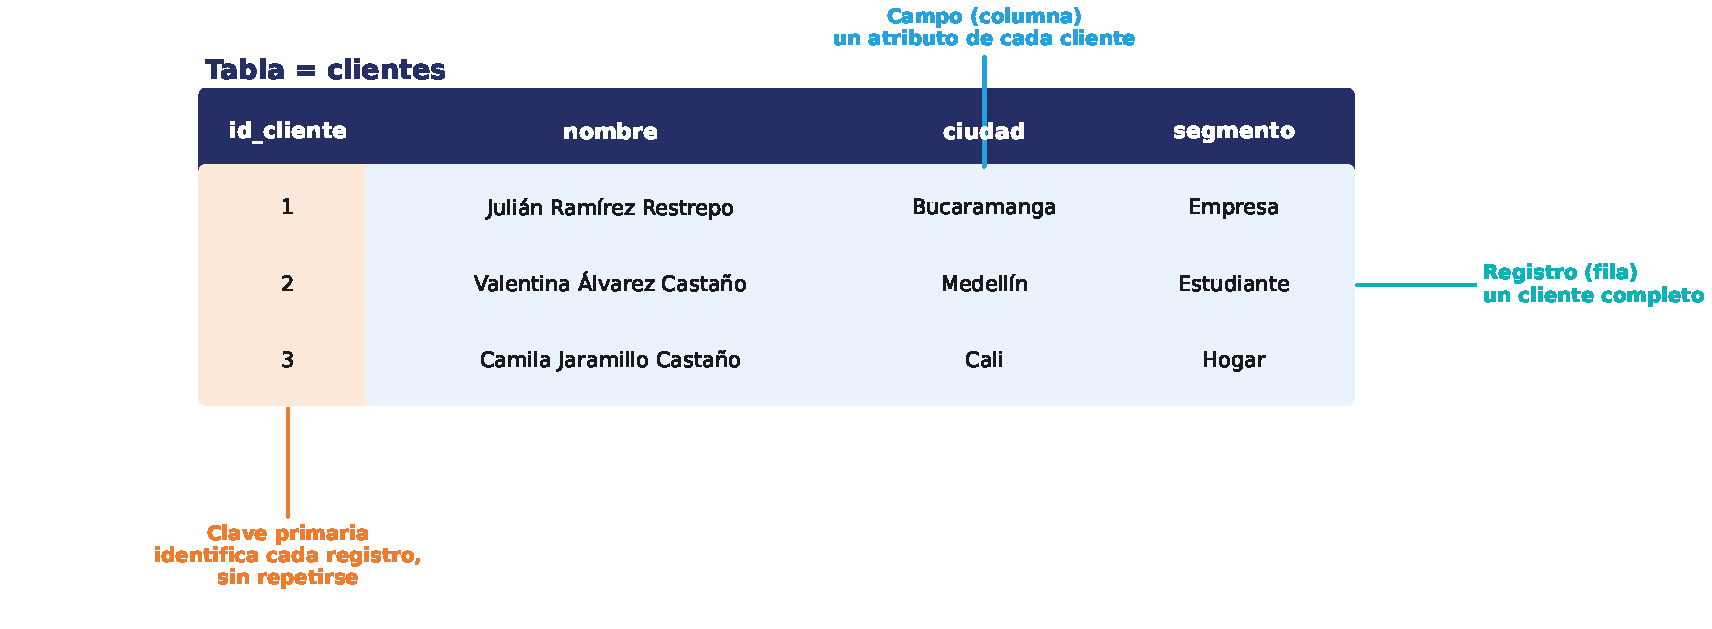
\includegraphics[width=0.92\textwidth]{figura_tabla_registro_campo.pdf}
  \end{center}
\end{frame}

\begin{frame}{Clave primaria y clave foránea}
  \small
  \textcolor{esumerOrange}{\textbf{Clave primaria (PK)}} — el campo que
  identifica \textbf{sin ambigüedad} cada registro de una tabla; no se
  repite y no puede quedar vacío. Ejemplo: \texttt{id\_cliente} en la
  tabla \texttt{clientes}.
  \vspace{0.2cm}
  \begin{block}{¿Por qué no usar el nombre como identificador?}
    \small Porque los nombres \textbf{se repiten} (dos clientes pueden
    llamarse igual) y \textbf{pueden cambiar} (un cliente puede corregir
    cómo está escrito su nombre). Un identificador numérico no tiene
    ninguno de esos problemas.
  \end{block}
  \vspace{0.2cm}
  \textcolor{esumerSky}{\textbf{Clave foránea (FK)}} — un campo que
  \textbf{apunta a la clave primaria de otra tabla}, y así conecta las dos
  tablas. Ejemplo: en \texttt{pedidos}, el campo \texttt{id\_cliente}
  reconoce \textit{a qué cliente} pertenece cada pedido.
\end{frame}

\begin{frame}{Esquema relacional: nuestra base de datos de práctica}
  \small
  Hoy trabajamos con \texttt{tienda.db}: una tienda en línea ficticia
  (``Tienda Andina''), con 5 tablas relacionadas entre sí mediante claves
  primarias y foráneas.
  \begin{center}
    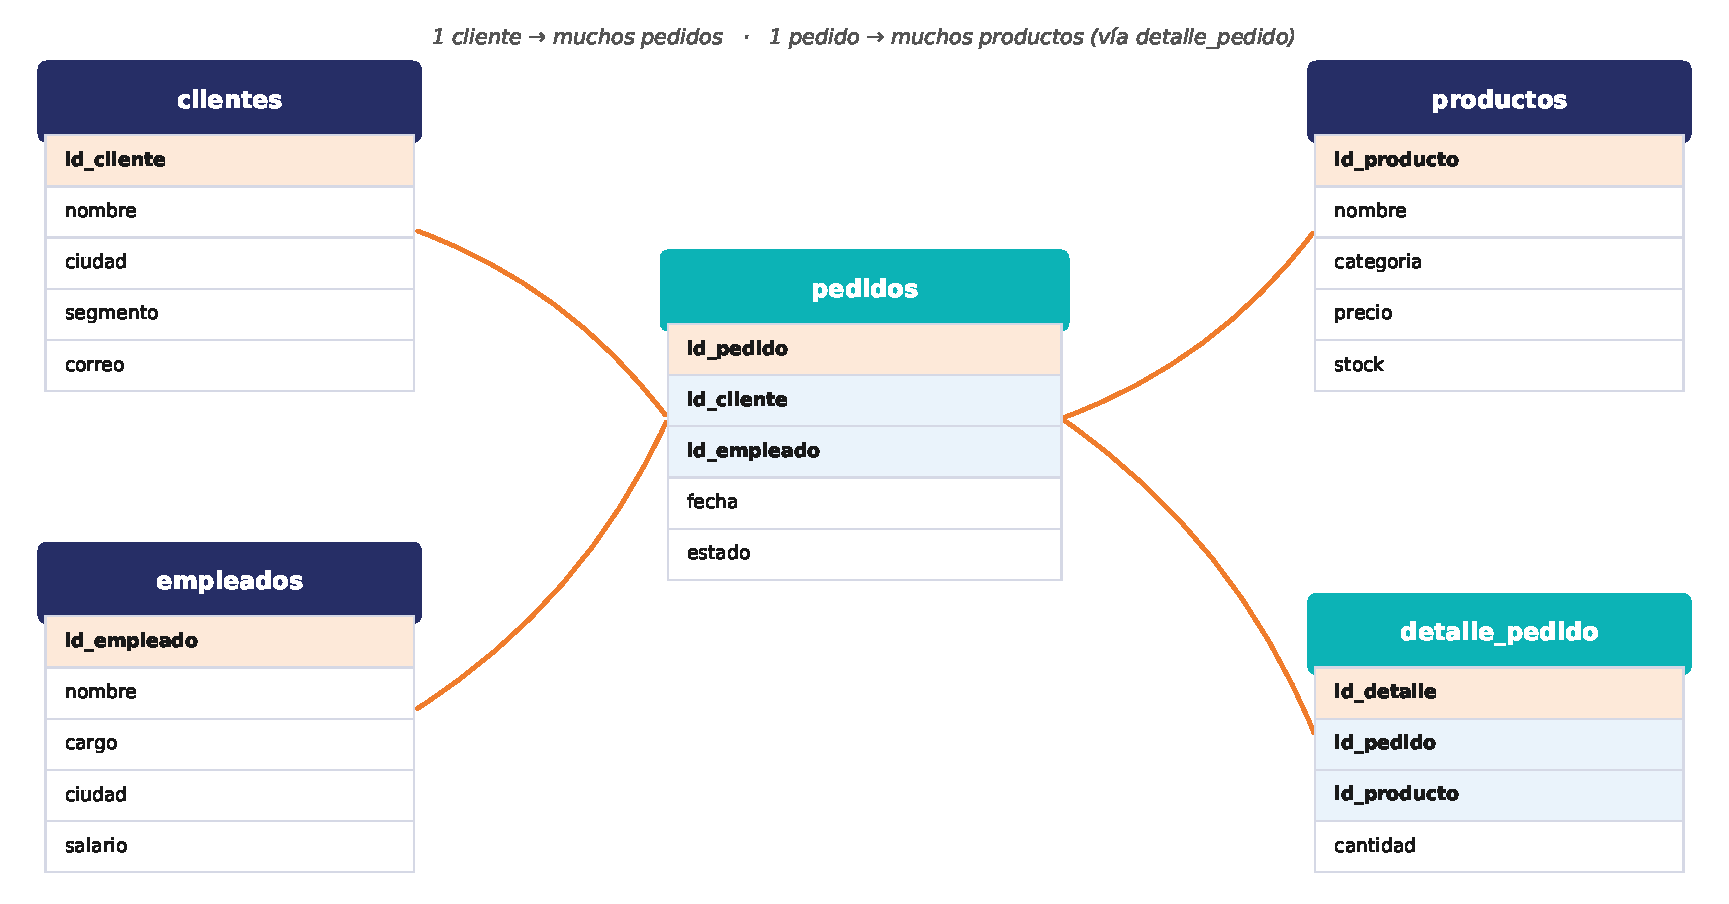
\includegraphics[width=0.88\textwidth,height=0.68\textheight,keepaspectratio]{figura_esquema_relacional.pdf}
  \end{center}
\end{frame}

\begin{frame}{¿Por qué aprender SQL si ya sabemos Python?}
  \small
  Porque \textbf{en el trabajo real casi nunca eliges tú dónde viven los
  datos}: muchas veces están en una base de datos, y para traerlos a
  Python (o a Power BI, Módulo 3) primero hay que saber pedírselos con SQL.
  \begin{exampleblock}{Lo que ya sabes de la Clase 4, con otro nombre}
    \small
    \begin{itemize}
      \item Filtrar filas de un \texttt{DataFrame} \;$\rightarrow$\; cláusula
        \texttt{WHERE}.
      \item Elegir columnas \;$\rightarrow$\; lo que escribes después de
        \texttt{SELECT}.
      \item \texttt{.sort\_values()} \;$\rightarrow$\; \texttt{ORDER BY}.
    \end{itemize}
  \end{exampleblock}
  \textbf{SQL} (\textit{Structured Query Language}) es el lenguaje estándar
  para hacerle preguntas a una base de datos relacional: se aprende una
  vez y sirve para (casi) cualquier motor (SQLite, PostgreSQL, MySQL, SQL
  Server\dots).
\end{frame}

% ============================================================
\section{Hora 2 — SQL básico}
% ============================================================
\begin{frame}[fragile]{Anatomía de una consulta SELECT}
  \small
  Toda consulta parte de la misma idea: de una tabla completa, pedimos
  \textbf{ciertas columnas} de \textbf{ciertas filas}.
  \begin{lstlisting}
SELECT nombre, ciudad
FROM clientes;
  \end{lstlisting}
  \vspace{-0.1cm}
  \begin{itemize}
    \small
    \item \texttt{SELECT} — \textbf{qué columnas} quiero ver.
    \item \texttt{FROM} — \textbf{de qué tabla} las quiero.
    \item Toda instrucción SQL termina en \textbf{punto y coma} (\texttt{;}).
  \end{itemize}
  \begin{alertblock}{El resultado de una consulta es siempre otra tabla}
    \small Así tenga una sola columna o una sola fila: el resultado de un
    \texttt{SELECT} se ve y se comporta como una tabla nueva.
  \end{alertblock}
\end{frame}

\begin{frame}[fragile]{Elegir columnas: nombradas o \texttt{*}}
  \small
  \begin{columns}[T,onlytextwidth]
    \column{0.5\textwidth}
    \textbf{Columnas específicas} (lo recomendado casi siempre):
    \begin{lstlisting}
SELECT nombre, precio
FROM productos;
    \end{lstlisting}
    \column{0.5\textwidth}
    \textbf{Todas las columnas}, con \texttt{*}:
    \begin{lstlisting}
SELECT *
FROM productos;
    \end{lstlisting}
  \end{columns}
  \vspace{0.2cm}
  \begin{block}{¿Por qué no usar siempre \texttt{*}?}
    \small Trae columnas que quizás no necesitas (más lento y más
    desordenado de leer), y si alguien le agrega una columna a la tabla
    mañana, tu consulta con \texttt{*} cambia de resultado sin que tú lo
    hayas pedido. Nombrar las columnas es más explícito y más seguro.
  \end{block}
\end{frame}

\begin{frame}{El orden en que se escribe vs. el orden en que se ejecuta}
  \small
  Un detalle que suele confundir al principio: SQL \textbf{no} ejecuta la
  consulta en el mismo orden en que la escribes.
  \begin{center}
    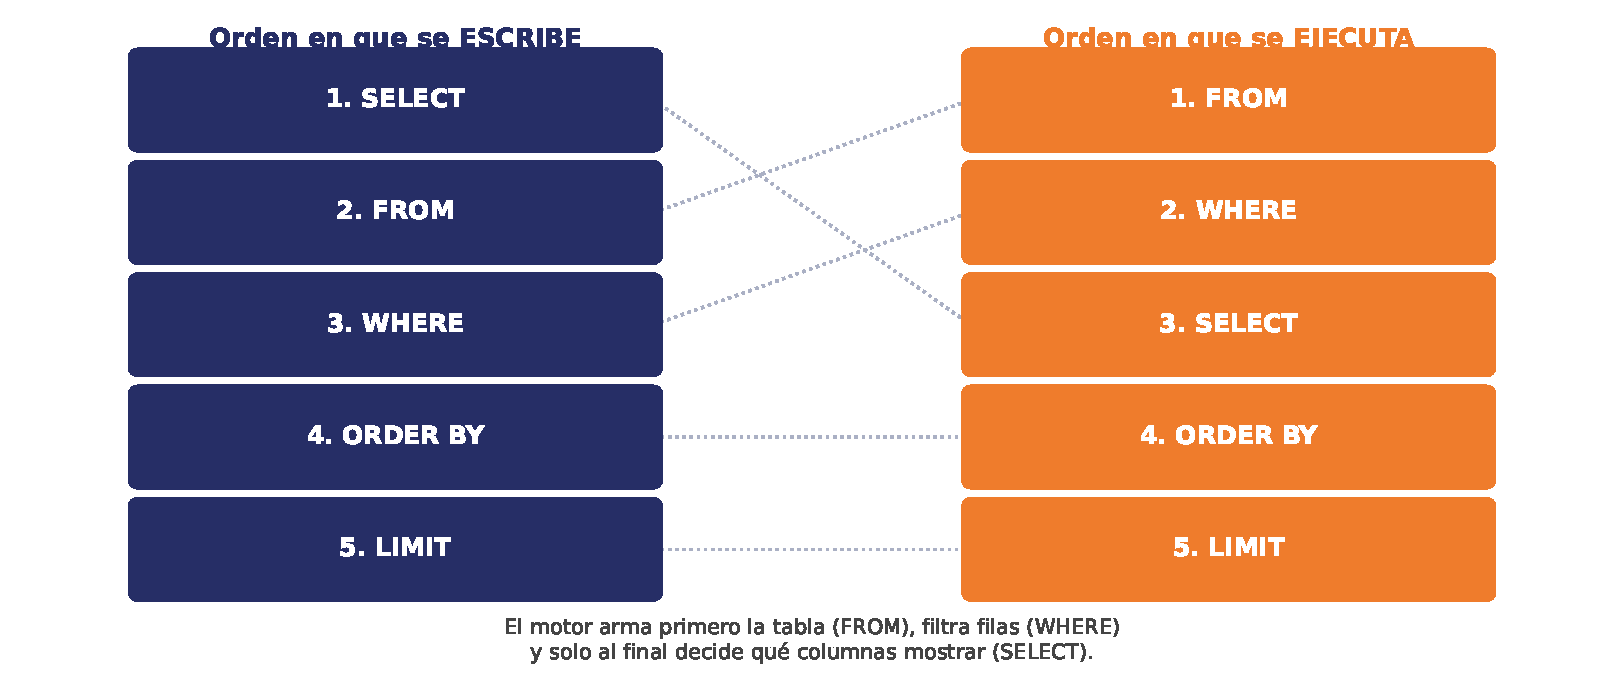
\includegraphics[width=0.8\textwidth,height=0.52\textheight,keepaspectratio]{figura_orden_logico_sql.pdf}
  \end{center}
  \small Por eso \texttt{WHERE} puede filtrar por una columna que ni
  siquiera aparece en el \texttt{SELECT}: el motor ya armó la tabla
  completa (\texttt{FROM}) y la filtró (\texttt{WHERE}) \textbf{antes} de
  decidir qué mostrar.
\end{frame}

\begin{frame}[fragile]{WHERE y operadores de comparación}
  \small
  \texttt{WHERE} filtra filas: solo pasan las que cumplen la condición
  (exactamente como \texttt{df[condición]} en pandas).
  \begin{center}
    \small
    \begin{tabular}{cl}
      \toprule
      \textbf{Operador} & \textbf{Significado} \\
      \midrule
      \texttt{=} & igual a \\
      \texttt{!=} \; ó \; \texttt{<>} & distinto de \\
      \texttt{>} \; / \; \texttt{<} & mayor que / menor que \\
      \texttt{>=} \; / \; \texttt{<=} & mayor o igual / menor o igual \\
      \bottomrule
    \end{tabular}
  \end{center}
  \begin{lstlisting}
SELECT nombre, ciudad
FROM clientes
WHERE ciudad = 'Medellín';
  \end{lstlisting}
  \small Los valores de texto van entre \textbf{comillas simples}
  (\texttt{'Medellín'}); los números, sin comillas (\texttt{precio > 200000}).
\end{frame}

\begin{frame}[fragile]{Ejemplo real: filtrar productos}
  \small
  Sobre la tabla \texttt{productos} de \texttt{tienda.db}:
  \begin{lstlisting}
SELECT nombre, precio
FROM productos
WHERE categoria = 'Tecnología' AND precio > 200000;
  \end{lstlisting}
  \begin{center}
    \small
    \begin{tabular}{lr}
      \toprule
      \textbf{nombre} & \textbf{precio} \\
      \midrule
      Portátil 14 pulgadas & 2\,450\,000 \\
      Monitor 24 pulgadas & 780\,000 \\
      Teclado mecánico & 245\,000 \\
      \bottomrule
    \end{tabular}
  \end{center}
  \small Dos condiciones unidas con \texttt{AND}: solo pasan las filas que
  cumplen \textbf{ambas} a la vez.
\end{frame}

\begin{frame}[fragile]{Operadores lógicos: AND, OR, NOT}
  \small
  \begin{itemize}
    \small
    \item \texttt{AND} — deben cumplirse \textbf{todas} las condiciones.
    \item \texttt{OR} — basta con que se cumpla \textbf{alguna}.
    \item \texttt{NOT} — invierte una condición.
  \end{itemize}
  \begin{alertblock}{Cuidado con mezclar AND y OR}
    \small SQL evalúa \texttt{AND} \textbf{antes} que \texttt{OR} (igual
    que la multiplicación antes que la suma). Si no es lo que quieres,
    usa \textbf{paréntesis} para dejarlo explícito.
  \end{alertblock}
  \begin{columns}[T,onlytextwidth]
    \column{0.5\textwidth}
    \small Sin paréntesis (ambiguo):
    \begin{lstlisting}
WHERE categoria = 'Hogar'
   OR categoria = 'Oficina'
  AND precio > 500000;
    \end{lstlisting}
    \column{0.5\textwidth}
    \small Con paréntesis (lo que sí queríamos):
    \begin{lstlisting}
WHERE (categoria = 'Hogar'
    OR categoria = 'Oficina')
  AND precio > 500000;
    \end{lstlisting}
  \end{columns}
  \small La primera versión trae \textbf{todo} Hogar (sin importar el
  precio) más Oficina caro; la segunda solo trae Hogar u Oficina, ambos
  por encima de \$500.000 — dos resultados distintos con las mismas
  palabras.
\end{frame}

\begin{frame}[fragile]{IN, BETWEEN, LIKE e IS NULL}
  \small
  Cuatro atajos muy usados para condiciones comunes:
  \begin{columns}[T,onlytextwidth]
    \column{0.5\textwidth}
    \textbf{IN} — pertenece a una lista:
    \begin{lstlisting}
WHERE ciudad IN
  ('Cali','Bogotá');
    \end{lstlisting}
    \textbf{BETWEEN} — dentro de un rango:
    \begin{lstlisting}
WHERE fecha BETWEEN
  '2026-03-01' AND '2026-03-31';
    \end{lstlisting}
    \column{0.5\textwidth}
    \textbf{LIKE} — coincide con un patrón
    (\texttt{\%} = cualquier texto):
    \begin{lstlisting}
WHERE nombre LIKE
  '%portátil%';
    \end{lstlisting}
    \textbf{IS NULL} — el campo está vacío:
    \begin{lstlisting}
WHERE correo IS NULL;
    \end{lstlisting}
  \end{columns}
  \vspace{0.2cm}
  \begin{block}{¿Por qué no \texttt{correo = NULL}?}
    \small Porque \texttt{NULL} significa ``valor desconocido'', y nada es
    \textit{igual} a algo desconocido — ni siquiera otro \texttt{NULL}. Por
    eso existe el operador especial \texttt{IS NULL} (y \texttt{IS NOT
    NULL}).
  \end{block}
\end{frame}

\begin{frame}[fragile]{Ordenar resultados: ORDER BY}
  \small
  \texttt{ORDER BY} ordena las filas del resultado por una o más columnas.
  Por defecto es ascendente (\texttt{ASC}); para descendente se agrega
  \texttt{DESC}.
  \begin{lstlisting}
SELECT nombre, precio
FROM productos
ORDER BY precio DESC;
  \end{lstlisting}
  \begin{center}
    \small
    \begin{tabular}{lr}
      \toprule
      \textbf{nombre} & \textbf{precio} \\
      \midrule
      Portátil 14 pulgadas & 2\,450\,000 \\
      Escritorio ajustable & 1\,150\,000 \\
      Monitor 24 pulgadas & 780\,000 \\
      \dots & \dots \\
      \bottomrule
    \end{tabular}
  \end{center}
\end{frame}

\begin{frame}[fragile]{Limitar resultados: LIMIT}
  \small
  \texttt{LIMIT} corta el resultado a las primeras \textit{n} filas — muy
  útil para explorar una tabla grande sin traerla completa, o para
  preguntas tipo ``los 3 productos más caros''.
  \begin{lstlisting}
SELECT nombre, precio
FROM productos
ORDER BY precio DESC
LIMIT 3;
  \end{lstlisting}
  \begin{center}
    \small
    \begin{tabular}{lr}
      \toprule
      \textbf{nombre} & \textbf{precio} \\
      \midrule
      Portátil 14 pulgadas & 2\,450\,000 \\
      Escritorio ajustable & 1\,150\,000 \\
      Monitor 24 pulgadas & 780\,000 \\
      \bottomrule
    \end{tabular}
  \end{center}
  \small Nota el orden real de ejecución (diapositiva anterior): primero
  se arma y filtra la tabla, \textbf{luego} se ordena, y \textbf{al final}
  se recorta con \texttt{LIMIT}.
\end{frame}

\begin{frame}[fragile]{Todo junto: WHERE + ORDER BY + LIMIT}
  \small
  Pregunta de negocio: \textit{``¿cuáles son los 3 productos con menos
  stock disponible?''}
  \begin{lstlisting}
SELECT nombre, stock
FROM productos
WHERE stock < 15
ORDER BY stock ASC
LIMIT 3;
  \end{lstlisting}
  \begin{center}
    \small
    \begin{tabular}{lr}
      \toprule
      \textbf{nombre} & \textbf{stock} \\
      \midrule
      Escritorio ajustable & 8 \\
      Archivador metálico & 10 \\
      Silla ergonómica & 12 \\
      \bottomrule
    \end{tabular}
  \end{center}
  \small Filtrar, ordenar y limitar se combinan todo el tiempo: la
  estructura siempre es \texttt{SELECT} \dots\ \texttt{FROM} \dots\
  \texttt{WHERE} \dots\ \texttt{ORDER BY} \dots\ \texttt{LIMIT}.
\end{frame}

% ============================================================
\section{Hora 3 — Laboratorio}
% ============================================================
\begin{frame}{Actividad práctica}
  \begin{alertblock}{Reto de la sesión}
    \small Practicar consultas de extracción y filtrado sobre
    \texttt{tienda.db}, una base de datos SQLite de una tienda en línea
    ficticia, con las mismas 5 tablas del esquema relacional que vimos hoy.
  \end{alertblock}
  \vspace{0.2cm}
  \small Dos caminos posibles, con la misma base de datos (\texttt{datos/tienda.db} en el repositorio del curso):
  \begin{itemize}
    \small
    \item \textbf{Google Colab} (como en la Clase 4): subes
      \texttt{tienda.db} con \texttt{files.upload()} y consultas con
      Python + \texttt{sqlite3} — cuaderno guiado paso a paso.
    \item \textbf{DBeaver} (opcional, si quieres una herramienta visual de
      base de datos): te conectas directamente al mismo archivo
      \texttt{tienda.db}, sin instalar ningún servidor.
  \end{itemize}
  \small No hace falta ningún servidor en la nube: SQLite vive en un solo
  archivo, y ese archivo es el que descargas y usas en cualquiera de los
  dos caminos.
\end{frame}

\begin{frame}{Producto esperado}
  \begin{exampleblock}{Entregable}
    \small Completar el cuaderno \texttt{lab-sql-basico.ipynb}: las
    consultas guiadas de cada sección, las actividades marcadas con
    \texttt{-- TODO}, y el reto final de 5 preguntas de negocio sobre
    \texttt{tienda.db} (equivalente en SQL al reto de la Clase 4 en
    pandas).
  \end{exampleblock}
  \small Guarda una copia del cuaderno en tu Google Drive antes de cerrar
  Colab (el archivo \texttt{tienda.db} que subiste es efímero, igual que
  vimos en la Clase 4).
\end{frame}

% ============================================================
\section{Cierre}
% ============================================================
\begin{frame}{Cierre y próxima sesión}
  \begin{itemize}
    \item Una base de datos relacional organiza la información en
      \textbf{tablas} conectadas por \textbf{claves primarias y foráneas}.
    \item \texttt{SELECT}, \texttt{FROM}, \texttt{WHERE}, \texttt{ORDER
      BY} y \texttt{LIMIT} responden, con otro lenguaje, las mismas
      preguntas de negocio que ya resolvías con pandas en la Clase 4.
    \item Próxima sesión, \textbf{Clase 6 — MasterClass}: recapitulación
      presencial de todo el Módulo 1 (estadística descriptiva, Python y
      SQL) antes de entrar al Módulo 2 (Pandas a fondo).
    \item En la \textbf{Clase 7} retomamos pandas, ahora para diagnóstico
      de calidad de datos: nulos, duplicados y tipos — muchas de las
      condiciones que hoy escribiste en \texttt{WHERE} (como \texttt{IS
      NULL}) reaparecen ahí.
  \end{itemize}
\end{frame}

{
\setbeamertemplate{footline}{}
\begin{frame}[plain]
  \begin{tikzpicture}[remember picture,overlay]
    \fill[esumerNavy] (current page.south west) rectangle (current page.north east);
    \node at (current page.center) {\color{white}\Huge\bfseries ¡Gracias!};
  \end{tikzpicture}
\end{frame}
}

\end{document}
